\chapter {Implementation of proof-of-concept}

With the solution analysis done, we can now start implementing proof-of-concept.
Before we start the implementation, we should define the goals we want to accomplish in the proof-of-concept.
These are the goals:
\begin{itemize}
    \item {Create or update nodes in a database}
    \item {Map LINQ to Cypher}
\end{itemize}

The main tools used are Visual Studio Code with multiple plugins like Copilot and \CS extension, which provides an IntelliSense.
Github is used as VCS. Code is available at this URL \url{https://github.com/TomStary/dotnet-neo4j-ogm} or in the appendix of this thesis.

To create a new project, we will use the following command in the terminal application: \texttt{dotnet new classlib} with parameters for the name of the project and others.
We also want to separate tests from the source code of the library, so we employ a file structure like this \ref{ref:fileStructure}.

\begin{figure}[H]
    \dirtree{%
        .1 dotnet-neo4j-ogm.
        .2 src.
        .3 {Neo4j.OGM}.
        .2 tests.
        .3 {Neo4j.OGM}.
        .2 {.gitignore} .
        .2 {Neo4j.OGM.sln}.
    }
    \caption{File structure}
    \label{ref:fileStructure}
\end{figure}

With the file structure prepared, we can begin our implementation. During the development of this
library, we will use \acrfull{tdd}. We will not go deep into this approach in this chapter,
as it will be described in the next chapter, but keep in mind that during development, \acrshort{tdd} was used as it is an excellent way to write and test libraries.

\section {Common infrastructure}

If we want to achieve set goals for proof-of-concept, we will need a common infrastructure like the implementation of \texttt{ISession} interface.
This interface can be described as an entry point for all of our operations with the database. It will handle both saving entities and creating DbSet
instances, which can be used to query over entities using LINQ.

For the session to work properly, we need to have a few things:

\begin{itemize}
    \item connection to the database
    \item domain metadata
\end{itemize}

The connection to a database and domain metadata can be acquired from the session's constructor or elsewhere. However,
the best solution is to use \texttt{SessionFactory} instead. Using a factory has many benefits. The client's code will not be responsible for
creating a connection to the database for each session instance. It will also have precalculated domain metadata. Another benefit is
that it will be possible to hide the concrete implementation of \texttt{ISession} interface.

Implementation of \texttt{SessionFactory} is simple, we create a class with constructor accepts three parameters:
\begin{itemize}
    \item {\texttt{string connectionString} - contains connection string to the database}
    \item {\texttt{IAuthToken token} - token created by \texttt{AuthTokens} class from Neo4j drivers library, used to authenticate connections to the database}
    \item {\texttt{params Assembly[] assemblies} - assemblies containing domain models}
\end{itemize}
Using the first two parameters, we can create \texttt{IDriver} instance, which will be used to create session instances. The third parameter is special
because the type of the parameter is prefixed with keyword \texttt{params}. It means we can call the constructor with as many instances of \texttt{Assembly} as we want
(we are limited only by language itself, which has a cap at $2^{14}$ parameters). From \CS documentation:
"No additional parameters are permitted after the \texttt{params} keyword in a method declaration, and only one params keyword is permitted in a method declaration." \cite{billwagner_params_nodate}

The assemblies refer to where domain models are located; we need from the client's code information which assemblies to scan using reflection to pick up classes
representing nodes and relationships. We need this data for the correct graph analysis during saving operations.

\subsection {Building metadata}

We described the importance of metadata, but how are we going to obtain them. We already have assemblies from client's code, that should contain
the domain model. We use these assemblies in \texttt{MetaData} class constructor. Here is an actual implementation of \texttt{MetaData} constructor:

\begin{listing}[H]
    \begin{minted}[
 frame=lines,
 framesep=2mm,
 baselinestretch=1,
 bgcolor=LightGray,
 linenos,
 breaklines
 ] {csharp}
/// <summary>
/// MetaData constructor.
/// </summary>
/// <param name="assemblies">Assemblies containing domain model.</param>
internal MetaData(params Assembly[] assemblies)
{
 _domainInfo = new DomainInfo(assemblies);
 Schema = new SchemaBuilder(_domainInfo).Build();
}
 \end{minted}
    \caption{\texttt{MetaData} constructor}
    \label{code:metadataconstructor}
\end{listing}

We can now see how are the assemblies passed to the \texttt{DomainInfo} constructor, inside this class, we going through all the assemblies
and scanning all classes obtained by the \texttt{Assembly.GetType} method. This method return an array of \texttt{Type} objects representing
all the types in the assembly. We can then check each \texttt{Type} if it has an annotation for the node or relationship. We check this by using
our custom extension methods for \texttt{Type}, \texttt{HasNodeAttribute} and \texttt{HasRelationshipEntityAttribute}. If the type has the annotation,
we are going to add it to the right dictionary, which will be used during building the schema. We can see how this is done in the following code:

\begin{listing}[H]
    \begin{minted}[
 frame=lines,
 framesep=2mm,
 baselinestretch=1,
 bgcolor=LightGray,
 linenos,
 breaklines
 ] {csharp}
/// <summary>
/// Check if given <see cref="Type" does have the <see cref="NodeAttribute"> applied as custom attribute.
/// </summary>
internal static bool HasNodeAttribute(this Type type)
 => type.GetCustomAttributes().Any(attribute => attribute is NodeAttribute);

/// <summary>
/// Check if given <see cref="Type" does have the <see cref="RelationshipEntityAttribute"> applied as custom attribute.
/// </summary>
internal static bool HasRelationshipEntityAttribute(this Type type)
 => type.GetCustomAttributes().Any(attribute => attribute is RelationshipEntityAttribute);
 \end{minted}
    \caption{\texttt{HasNodeAttribute} and \texttt{HasRelationshipEntityAttribute} extension methods}
    \label{code:typeextensions}
\end{listing}

\subsection{\texttt{inline} keyword}

Keen reader might caught it up, but in last two code examples \ref{code:metadataconstructor} and \ref{code:typeextensions} we used the keyword \texttt{internal}
as an access modifier to the defined methods. This access modifier makes methods, classes, and properties available only inside the assembly. More on this subject
can be read at the official documentation of \CS language, URL: \url{https://docs.microsoft.com/en-us/dotnet/csharp/language-reference/keywords/internal}.

\subsection {Building schema}

Building schema is the last step in creating metadata for the client's domain model.
We use \texttt{SchemaBuilder} class to build the schema. We need to pass the \texttt{DomainInfo} instance to the \texttt{SchemaBuilder} constructor.
At the start we create new \texttt{Schema} instance, which is our concrete implementation of \texttt{ISchema} interface.

\texttt{SchemaBuilder.Build} method is responsible for building the schema. It does that by iterating over nodes and relationships and adding them to \texttt{Schema} instance
using \texttt{ISchema.AddNode} and \texttt{ISchema.AddRelationship} methods. The resulting schema is then returned.

We now have both schema and driver for creating the session. We will store both of them inside \texttt{SessionFactory} instance
and use them every time the session is created. To help client's code to manage instances of \texttt{SessionFactory} we will create an extension
of \texttt{IServiceCollection} which is a component of .NET responsible for managing the \acrfull{dic}. The lifetime of the \texttt{SessionFactory} is
a singleton, meaning that only one instance will be created during the runtime of the application. The extension implementation is shown here \ref{code:collectionextension}.

\begin{listing}[H]
    \begin{minted}[
 frame=lines,
 framesep=2mm,
 baselinestretch=1,
 bgcolor=LightGray,
 linenos,
 breaklines
 ] {csharp}
/// <summary>
/// Try and register the Neo4j OGM services in the DI container.
/// </summary>
public static IServiceCollection AddNeo4jOGMFactory(
 this IServiceCollection serviceCollection,
 string connectionString,
 IAuthToken authToken,
 params Assembly[] assemblies
 )
{
 serviceCollection.TryAddSingleton(
 new SessionFactory(connectionString, authToken, assemblies));
 return serviceCollection;
}
 \end{minted}
    \caption{\texttt{IServiceCollection} extension method}
    \label{code:collectionextension}
\end{listing}

With this extension method done, we have finished the common infrastructure, and we can now go and start implementing our
goals from the beginning of this chapter.

\section{Create or update nodes in a database}

\begin{listing}[H]
    \begin{minted}[
 frame=lines,
 framesep=2mm,
 baselinestretch=1,
 bgcolor=LightGray,
 linenos,
 breaklines
 ] {csharp}
/// <summary>
/// Save entity or list of entities to the database.
/// </summary>
public async Task SaveAsync<TEntity>(TEntity entity) where TEntity : class
{
 CheckDisposed();

 // tranform entity/entities into array
 IEnumerable<TEntity> objects;
 if (typeof(IEnumerable).IsAssignableFrom(entity.GetType()))
 {
 objects = (IEnumerable<TEntity>)entity;
 }
 else
 {
 objects = new[] { entity };
 }

 // map objects into a graph and creates statements
 foreach (var item in objects)
 {
 _entityGraphMapper.Map(item, -1);
 }

 // execute statements
 await ExecuteSave(_entityGraphMapper.CompilerContext());
}
 \end{minted}
    \caption{Internal implementation of save operation}
    \label{code:saveimpl}
\end{listing}

From the snippet above \ref{code:saveimpl} is an actual implementation of the save operation inside \texttt{ISession} concrete implementation.
We are going to use the \texttt{EntityGraphMapper} class to map the entity/entities into a structure that will be translated into
\texttt{IStatement} objects which represent statements that will be executed in the database. During mapping, we will also note the relationships between nodes
using information from \texttt{MetaData} object we built for this purpose. This whole concept is borrowed from
the official implementation of the Neo4j-\acrshort{ogm} library for Java.

\subsection{\texttt{EntityGraphMapper}}

The \texttt{EntityGraphMapper} is responsible for mapping the entities that will be translated into Cypher, as was stated in the paragraph before.
The resulting structure of this translation is saved inside a compiler context. The compiler context is a container for all the information
used during mapping and generating Cypher queries. It tracks visited nodes as well as visited relationships.

Inside the \texttt{ICompilerContext} is saved the instance of compiler, in this case it is \texttt{IMultiStatementCypherCompiler},
which is responsible for generating create and update Cypher queries. This compiler is used inside the\linebreak\texttt{Session.ExecuteSave} method.

\subsection{\texttt{IMultiStatementCypherCompiler}}

\begin{listing}[H]
    \begin{minted}[
 frame=lines,
 framesep=2mm,
 baselinestretch=1,
 bgcolor=LightGray,
 linenos,
 breaklines
 ] {csharp}
public interface IMultiStatementCypherCompiler
{
 CompilerContext Context { get; }
 NodeBuilder CreateNode(long id);
 IEnumerable<IStatement> CreateNodesStatements();
 NodeBuilder ExistingNode(long id);
 RelationshipBuilder ExistingRelationship(long relId, string type);
 IEnumerable<IStatement> GetAllStatements();
 bool HasStatementDependentOnNewNode();
 RelationshipBuilder NewRelationship(string type);
 RelationshipBuilder NewRelationship(string type, bool mapBothDirections);
 void UseStatementFactory(IStatementFactory statementFactory);
}
 \end{minted}
    \caption{\texttt{IMultiStatementCypherCompiler} interface}
    \label{code:IMultiStatementCypherCompiler}
\end{listing}

This interface defines a set of methods needed for preparing and generating \texttt{IStatement} instances that will then be executed on the database.
The \texttt{NodeBuilder} and \texttt{RelationshipBuilder} classes are what used inside\linebreak\texttt{EntityGraphMapper} and are the building blocks for
\texttt{IStatement} instances.

\subsection{\texttt{IStatement}}

The \texttt{IStatement} was mentioned multiple times. It is a simple wrapper around a string containing the Cypher query and dictionary of parameters
used in the query. These two values can then be used to generate \texttt{Query} object from Neo4j.Driver library. \texttt{Query} is used by
Neo4j.Driver in their transaction implementation.

\section{Mapping LINQ to Cypher}

The process of mapping LINQ to Cypher can be divided into these steps:
\begin{itemize}
    \item {prepare LINQ query}
    \item {map LINQ to our expression tree}
    \item {map our expression tree into Cypher}
    \item {map result from database into result object.}
\end{itemize}
We will look at each step and show some of the implementations.

\subsection{Prepare LINQ query}

Before we translate the query, we have to prepare our LINQ query. Preparation starts with the definition of the asynchronous method in the \texttt{DbSet<T>} class
or the \texttt{IQueryable<T>} extension of an asynchronous method. The best example of this definition would be method \texttt{FindAsync} as it is defined
in the \texttt{DbSet<T>} class, but it also uses an extension method for \texttt{IQueryable<T>} interface. The reason behind using asynchronous methods is
the implementation of \texttt{IDriver} which has only asynchronous methods for working with transactions.

Apart from the checks of the key values, the method will also create a lambda expression that will be translated into the \texttt{WHERE} statement
in the Cypher query. This lambda expression is then passed to the \texttt{FirstOrDefaultAsync} method, which is an extension of the \texttt{IQueryable<T>} interface
as we discussed above. The example below \ref{code:dbSetFindAsync} shows the exact implementation of the \texttt{DbSet<T>.FindAsync} method.
Inside the extension method of\linebreak\texttt{FirstOrDefaultAsync}, we are calling the \texttt{IAsyncQueryProvider.ExecuteAsync<T>} method. This method
is responsible for translation and execution of the query.

\begin{listing}[H]
    \begin{minted}[
 frame=lines,
 framesep=2mm,
 baselinestretch=1,
 bgcolor=LightGray,
 linenos,
 breaklines
 ] {csharp}
public virtual Task<TEntity?> FindAsync(params object?[]? keyValues)
{
 if (keyValues == null
 || keyValues.Any(key => key == null))
 {
 return Task.FromResult<TEntity?>(default);
 }

 var keyProperties = typeof(TEntity).GetProperties()
 .Where(property => property.GetCustomAttribute<KeyAttribute>() != null)
 .ToArray();

 if (keyProperties.Length != keyValues.Length)
 {
 throw new ArgumentException("Incorrect number of key values");
 }

 return this.FirstOrDefaultAsync(BuildLambda(keyProperties, new ValueBuffer(keyValues)));
}
\end{minted}
    \caption{\texttt{DbSet<T>.FindAsync} implementation}
    \label{code:dbSetFindAsync}
\end{listing}

\subsection{Expression visitors}

Our goal is to create a custom expression tree that would copy a Cypher with additional information about the mapping of the result.

First of all, we will introduce such classes to which we want to translate our LINQ expression tree \ref{fig:cypherexpression}.

\begin{figure}[H]
    \centering
    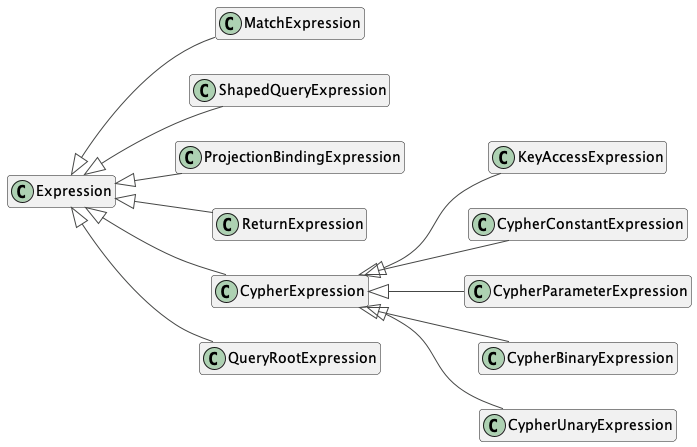
\includegraphics[width=\textwidth]{content/Cypher Expressions.png}
    \caption{Custom classes for translating LINQ expression tree}
    \label{fig:cypherexpression}
\end{figure}

To translate LINQ query to our custom expression tree, we will use the \texttt{QueryableMethodTranslationExpressionVisitor} class.
This class implements the \texttt{ExpressionVisitor} abstract class from LINQ. Our query is starts as \texttt{QueryRootExpression} which is
translated into \texttt{ShapedQueryExpression}. The \texttt{ShapedQueryExpression} contains the \texttt{MatchExpression} and\linebreak\texttt{EntityShaperExpression}
expression. This translation is done inside\linebreak\texttt{VisitExtension} method which is called for each expression marked with \texttt{ExpressionType.Extension}
as their \texttt{NodeType} property.

To set up \texttt{MatchExpression}, we are using a method \texttt{VisitMethodCall} which visits the children of the \texttt{MethodCallExpression}.
This method translates calls like \texttt{FirstOrDefault} from LINQ library. Inside this method the \texttt{WHERE} clause is translated as well
as \texttt{MatchExpression} other properties like\linebreak\texttt{MatchPattern.Limit}. Also the \texttt{ReturnExpression} is created inside this method.

The result of \texttt{Visit} method is a \texttt{ShapedQueryExpression} which contains the \texttt{MatchExpression}
with \texttt{ReturnExpression} and other predicates and expressions. This expression is now ready to be translated into Cypher query.

The visitor responsible for the actual translation to Cypher is\linebreak\texttt{CypherExpressionVisitor}. Inside this expression visitor,
we declare methods that corresponds with our custom classes, like \texttt{VisitCypherBinary} or \texttt{VisitMatch}. Each of these methods translates part of the expression
tree into a Cypher query. When the translation is done, the generated query is used in our custom enumerator, which enumerates the result from the database. This enumerator
is implemented inside \texttt{QueryingEnumerable<T>} class.

With the enumerator done, and the query generated, we need to execute our custom expression tree to get the result we want. To do this, we will use another visitor. In this case, this visitor needs to visit our\linebreak\texttt{ShapedQueryExpression} and create a right call that enumerates and returns the result.
The name of the class is\linebreak\texttt{ShapedQueryCompilingExpressionVisitor} and it checks if the result should be resulting in a single value or collection.
Inside, this visitor has also defined a custom lambda function, which will take the insides of\linebreak\texttt{ProjectionBindingExpression} and translate them to our result object.

\section{Summary}

This chapter was about implementing the library we designed in the chapter before. We described the structure of our project and then implemented
two critical goals of our proof-of-concept. With the first goal, we implemented the save operation for entities. We used metadata with information about graph
schema to properly create nodes and relationships. The second goal was mapping LINQ to Cypher query and extracting results from the database structure; we had to implement our own expressions structure to transform the expression tree so that we would be able to translate it to Cypher query.


